 \documentclass[conference]{IEEEtran}
\IEEEoverridecommandlockouts
% The preceding line is only needed to identify funding in the first footnote. If that is unneeded, please comment it out.
\usepackage{cite}
\usepackage{amsmath,amssymb,amsfonts}
\usepackage{algorithmic}
\usepackage{graphicx}
\usepackage{float} 
\usepackage{subfigure} 
\usepackage{textcomp}
\usepackage{xcolor}
\def\BibTeX{{\rm B\kern-.05em{\sc i\kern-.025em b}\kern-.08em
    T\kern-.1667em\lower.7ex\hbox{E}\kern-.125emX}}
\begin{document}

\title{System Model and Design: Tripedia\\
}

\author{\IEEEauthorblockN{Yulin Zhang}
\IEEEauthorblockA{\textit{7th Group} \\
\textit{Software Engineering}\\
Montreal, Canada \\
silveralex2023820@gmail.com}
\and
\IEEEauthorblockN{Yuhang Chen}
\IEEEauthorblockA{\textit{7th Group} \\
\textit{Software Engineering}\\
Montreal, Canada \\
yuhang.chen@mail.concordia.ca}
\and
\IEEEauthorblockN{Jiaxi Yang}
\IEEEauthorblockA{\textit{7th Group} \\
\textit{Software Engineering}\\
Montreal, Canada \\
yjxyang2@outlook.com}
\and
\IEEEauthorblockN{Boyang Wang}
\IEEEauthorblockA{\textit{7th Group} \\
\textit{Software Engineering}\\
Montreal, Canada \\
wangboyang0626@outlook.com}
}

\maketitle


\begin{figure*}[htbp]
\centerline{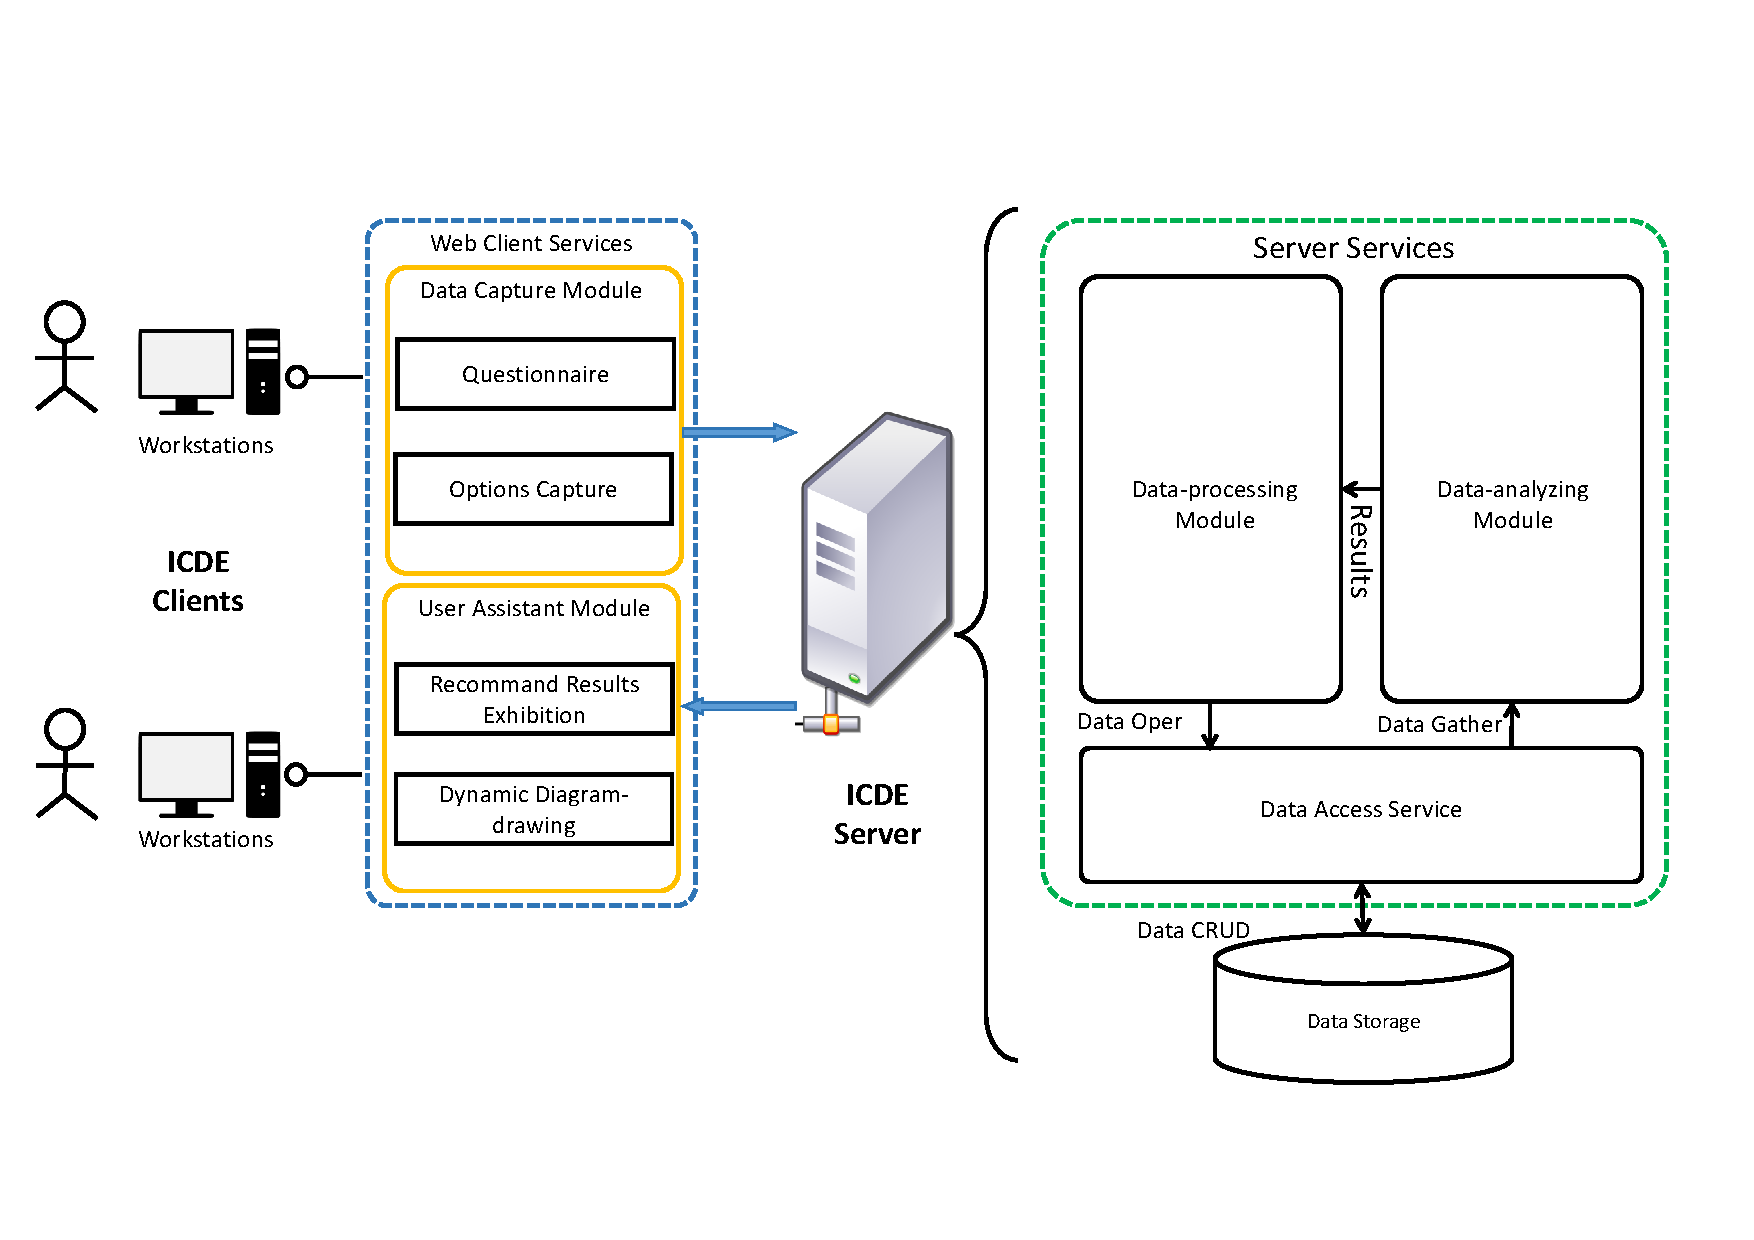
\includegraphics[width=0.9\textwidth]{Architecture.pdf}}
\caption{The architecture graph of Tripedia.}
\label{fig1}
\end{figure*}


\section{\textbf{The Agile Process}}


\subsection{\textbf{Team Setup}}



\subsection{\textbf{Association between User Stories and Sub-requirements}}

\subsection{\textbf{The Scrum Sprint Cycle}}

\subsubsection{\textbf{Review Work to be done}}


\subsubsection{\textbf{Product Backlog}}

\subsubsection{\textbf{Sprint Plan}}



\subsubsection{\textbf{Sprint Backlog}}

\subsubsection{\textbf{Sprint Process}}

\subsubsection{\textbf{Sprint Review}}


\section{\textbf{Architecture}}


\subsection{\textbf{Architecture Design in Overall Level}}

As shown in Figure\ref{fig1}, the ICDE system architecture mainly contains two parts: client and server. Based on the limited server hardware equipment, we implement the data analysis logic as a single module in the server, which stands for ICDE 3rd Party Applications. 

In the client part, we implement Tripedia's client logic based on the web. The web client service is mainly divided into two parts: the Data Capture Module and User Assistant Module. The Data Capture Module captures the user's behavior and personal information through questionnaires and behavior captures, and transmits the relevant information to the server. The User Assistant Module is responsible for displaying processed data sent by the server, such as recommendation results and data analysis results, which help users make decisions easily.

On the server side, we will develop three modules to implement the backbone of the ICDE system: Data-processing Module, Data-analyzing Module, and Data Access Service. The Data Access Service, as the median layer for database access, provides a unified database interface (deletion, modification, query, etc) for the Data-processing Module and the Data-analyzing module. The Data-processing Module is responsible for the basic logic of the server, such as registration, login, search, data preprocessing, and other interaction logic with the client. The Data-analyzing Module accesses the data in the database through the Data Access Service to perform data analysis and returns the analysis results to the Data-processing Module.

To sum up, Tripedia's architecture is a standard ICDE system. The Client part includes a Data Capture Service to collect user behavior and information and transmit relevant data to the server. The Data-processing Module in the Servers section is responsible for implementing the interactive logic of the server; the Data Access Service provides a unified data access interface; the Data-analyzing Module serves as the core of the ICDE system to analyze user data and feedback the analysis results to the user through the server to provide User Assistance Service.


\subsection{\textbf{Architecture Design in User Requirements Level}}

In this section, we will discuss the design of the tasks of the Tripedia. For a clearer structural presentation, we consider the choice of task description granularity. A small task granularity can not take on the task of showing interactions among multiple objects. A large task granularity may lose the meaning of the task design. Therefore, we merged some sub-requirements into a single task. We try to show the relationships among objects as much as possible while ensuring appropriate granularity. 


\section{\textbf{Modeling and Design}}


\subsection{\textbf{Task: Searching Data from Database }}


\subsubsection{\textbf{Task Conext }}

\begin{figure}[htbp]
	\centerline{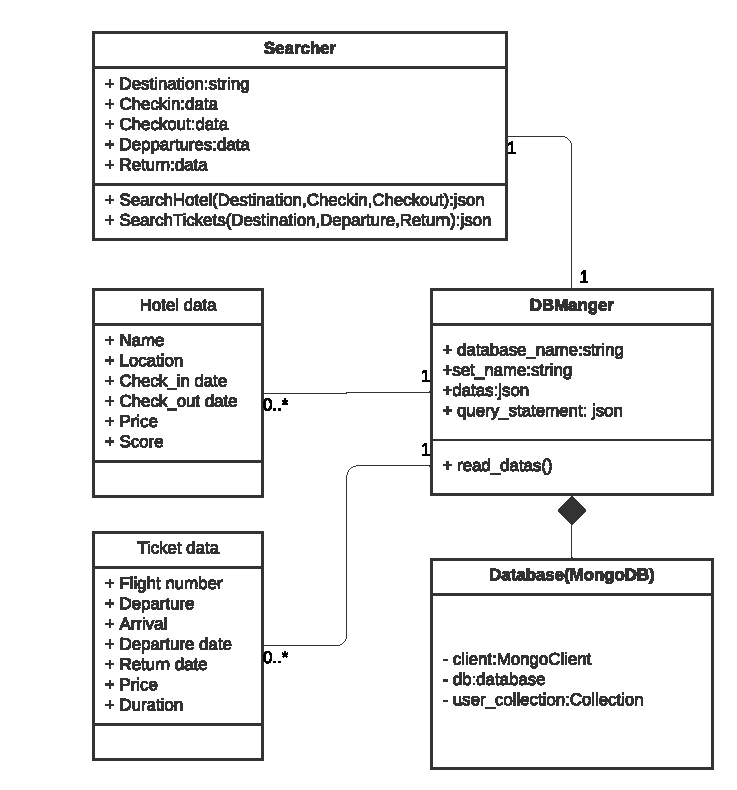
\includegraphics[width=0.5\textwidth]{image/searching hotel class1.pdf}}
	\caption{Class diagram of Searching data from database }
	\label{class1}
\end{figure}

\subsubsection{\textbf{Structural Conext }}

\begin{figure}[htbp]
	\centerline{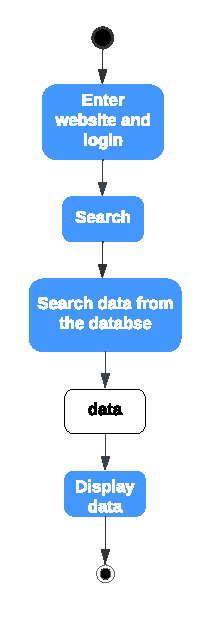
\includegraphics[width=0.18\textwidth]{image/searching hotel activity1.pdf}}
	\caption{Activity diagram of Searching data from database }
	\label{activity1}
\end{figure}


\subsubsection{\textbf{Interaction Conext }}

\begin{figure}[htbp]
	\centerline{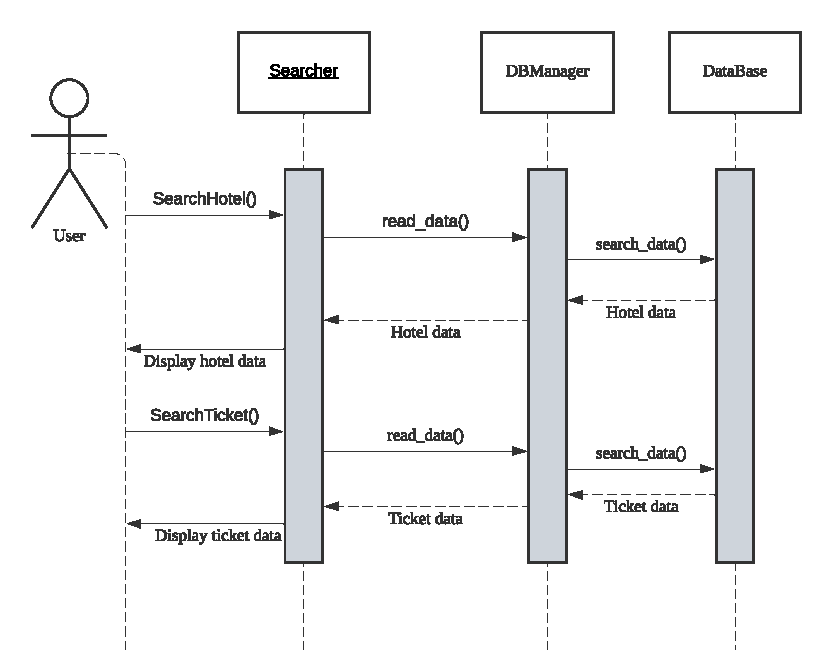
\includegraphics[width=0.5\textwidth]{image/searching hotel sequence1.pdf}}
	\caption{Sequence diagram of Searching data from database }
	\label{sequence1}
\end{figure}

\subsubsection{\textbf{Behavior Conext }}

\begin{figure}[htbp]
	\centerline{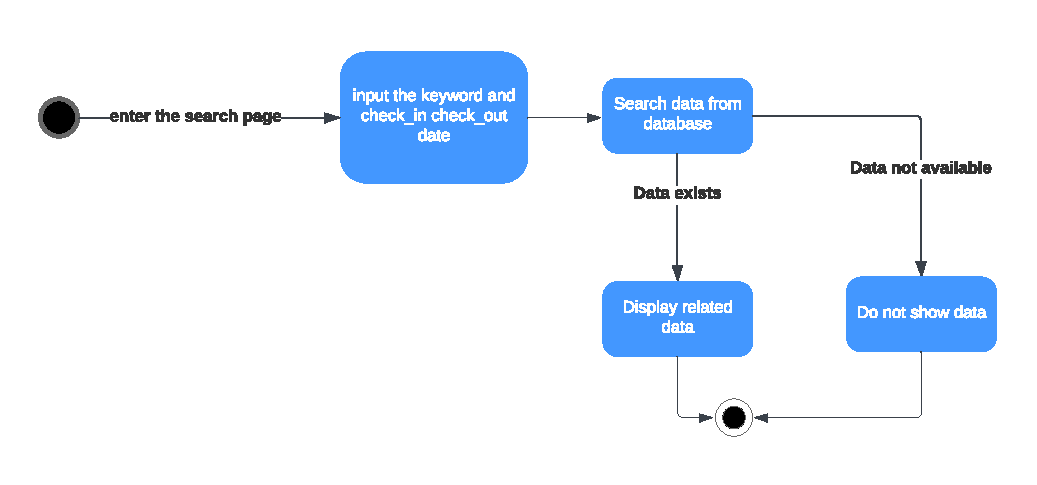
\includegraphics[width=0.5\textwidth]{image/searching hotel statement1.pdf}}
	\caption{Statement diagram of Searching data from database }
	\label{statement1}
\end{figure}

\subsection{\textbf{Task: Crawler searching }}


\subsubsection{\textbf{Task Conext }}

\begin{figure*}[htbp]
	\centerline{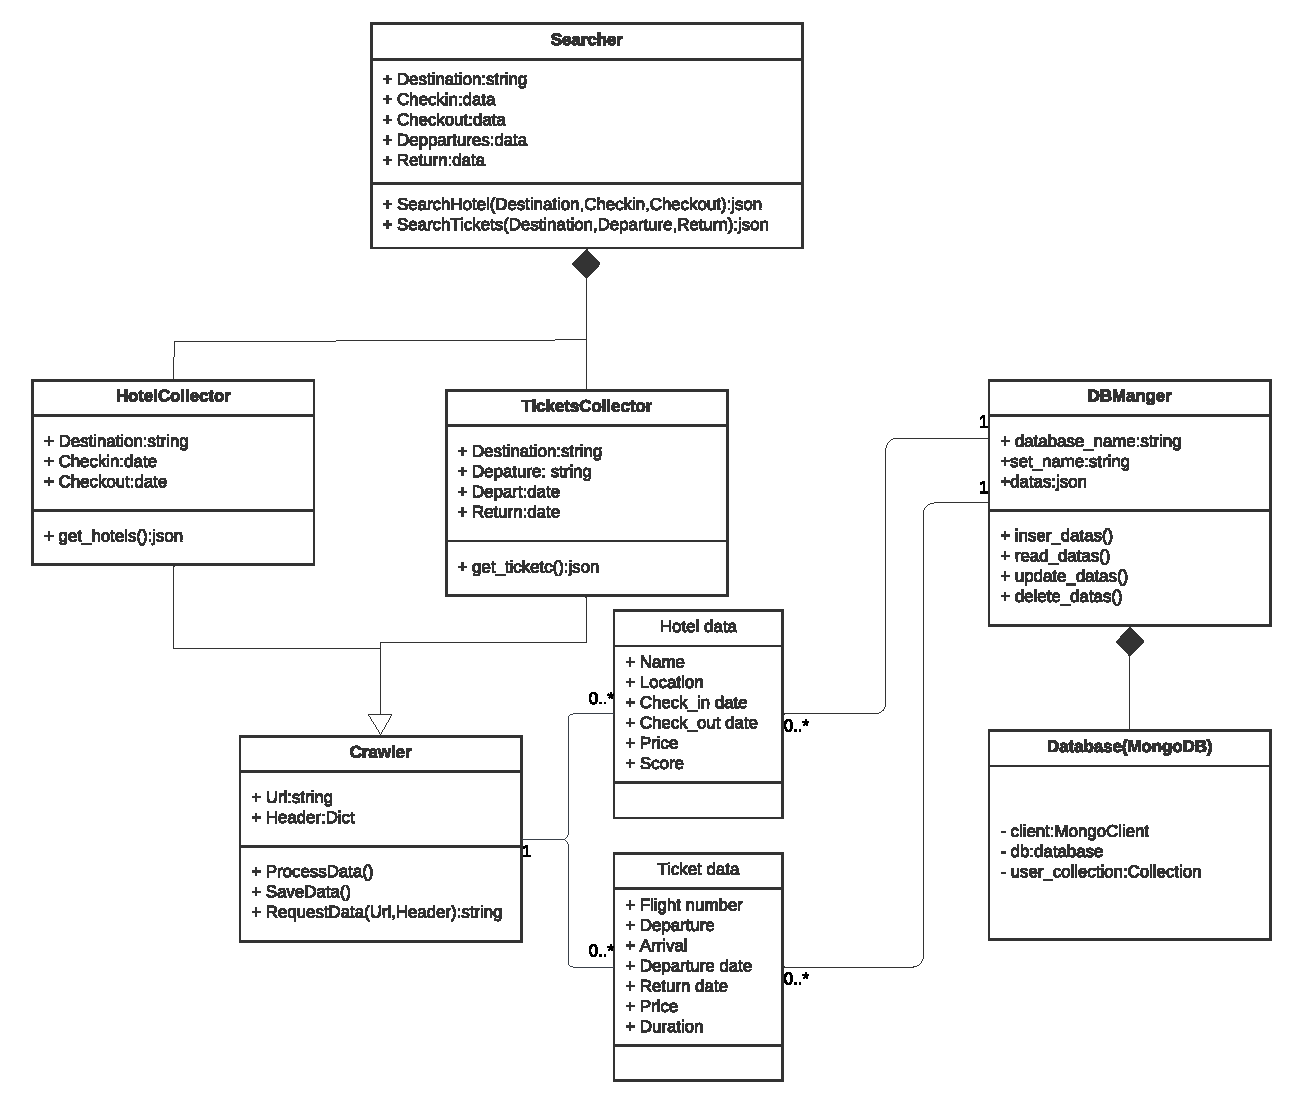
\includegraphics[width=0.9\textwidth]{image/crawler search class1.pdf}}
	\caption{Class diagram of Crawler searching }
	\label{class1}
\end{figure*}

\subsubsection{\textbf{Structural Conext }}

\begin{figure}[htbp]
	\centerline{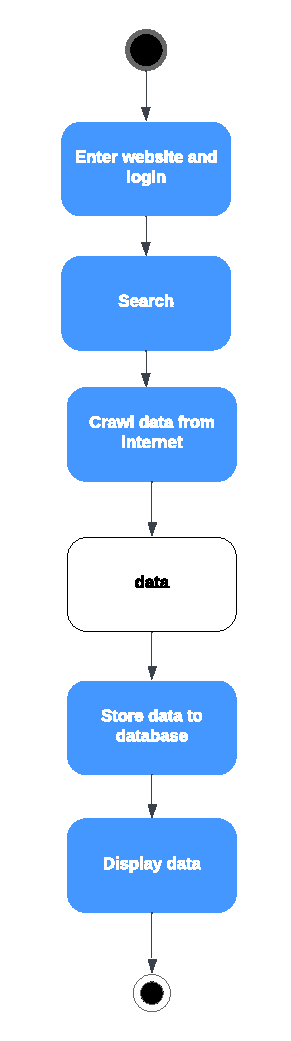
\includegraphics[width=0.16\textwidth]{image/crawler activity1.pdf}}
	\caption{Activity diagram of Crawler searching }
	\label{activity1}
\end{figure}


\subsubsection{\textbf{Interaction Conext }}

\begin{figure}[htbp]
	\centerline{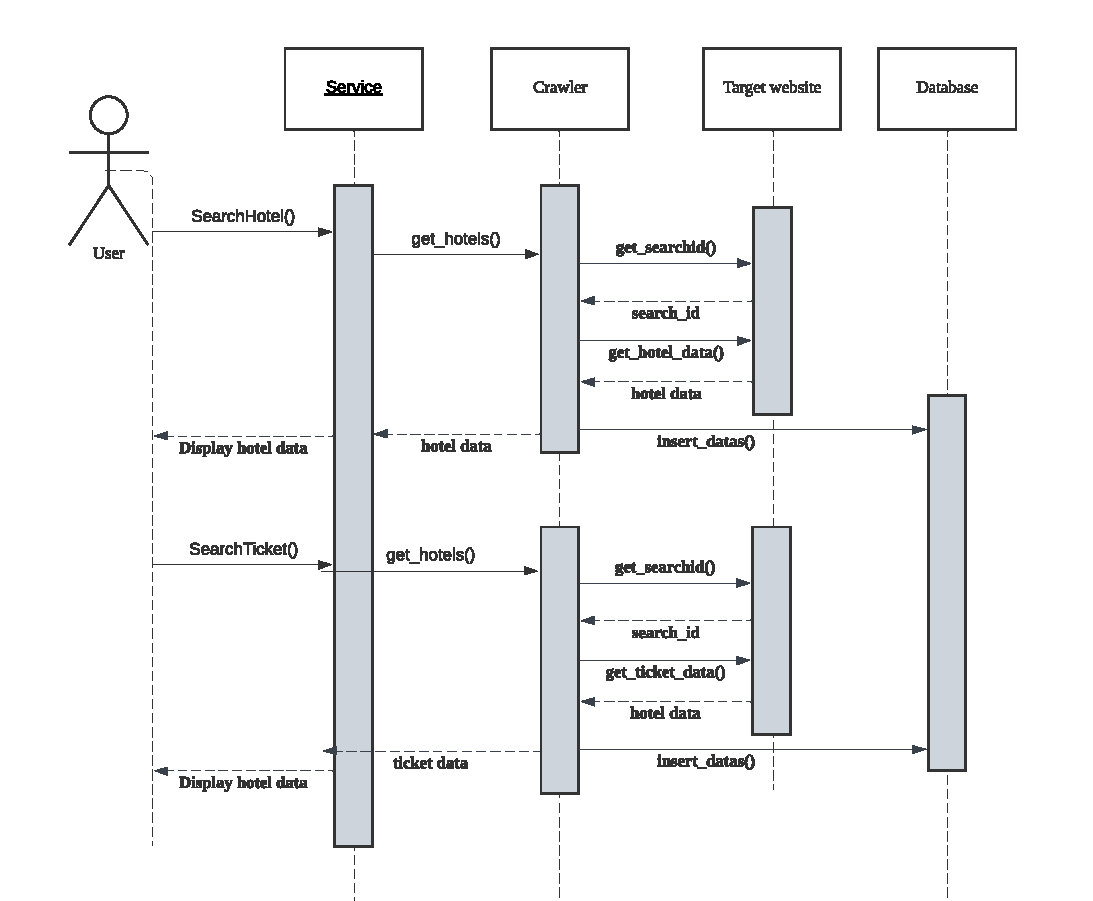
\includegraphics[width=0.5\textwidth]{image/crawler searching sequence1.pdf}}
	\caption{Sequence diagram of Crawler searching }
	\label{sequence1}
\end{figure}

\subsubsection{\textbf{Behavior Conext }}

\begin{figure}[htbp]
	\centerline{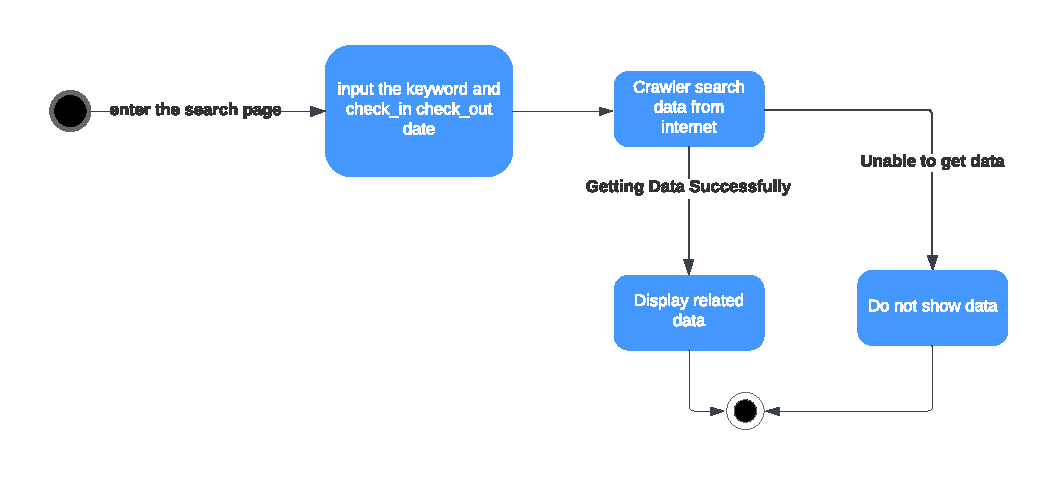
\includegraphics[width=0.5\textwidth]{image/crawler searching statement1.pdf}}
	\caption{Statement diagram of Crawler searching }
	\label{statement1}
\end{figure}



\subsection{\textbf{Task: The Analysis Diagram}}


\subsubsection{\textbf{Task Conext }}

\textbf{}

\begin{figure*}[htbp]
\centerline{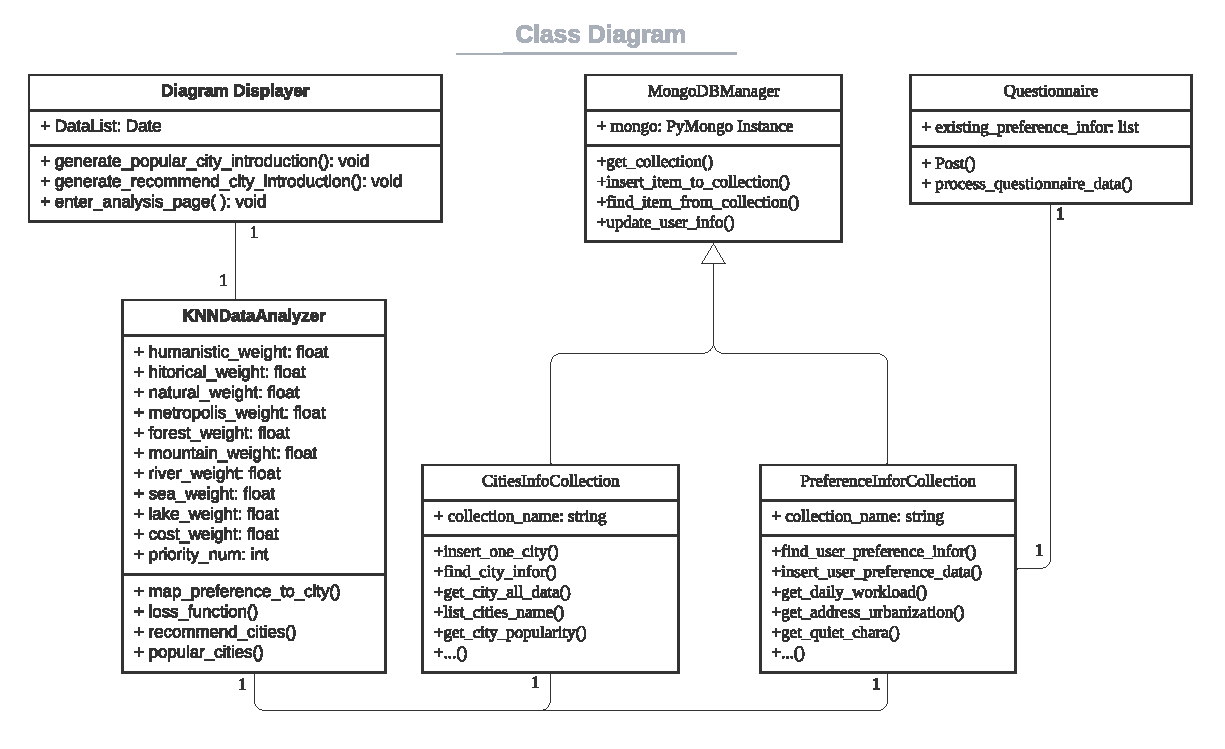
\includegraphics[width=1.0\textwidth]{diagram_structual_context.pdf}}
\caption{The class diagram of analysis diagram task.}
\label{fig_diagram_class}
\end{figure*}

The class diagram in Figure \ref{fig_diagram_class} shows the relationships among the analyzer, questionnaire, displayer, and database manager. 

For high efficiency and reusability, we designed a mediate layer for accessing the database. The MongoDBManager is a base class in the database interface, which encapsulates the Mongo Database interface. The Mongo DB Manager can be generalized as the Cities Information Collection and Preference Information Collection. The Cities Information Collection has extended with some class functions related to the city information. Meanwhile, the Preference Information Collection has extended with some class functions related to user preference information.

The Questionnaire class is responsible for catching user's preference information. A global Preference Infor Collection class instance provides the database interface for the data processing function in the Questionnaire class. Hence, the Preference Information Collection is associated with the Questionnaire.

On the other side of the class diagram, the diagram displayer performs the issues about analysis data displaying, which is based on the data analyzed by the KNNDataAnalyzer. The KNN Data Analyzer compares each city data entry with the user's preference and decides which city is the most appropriate recommendation. In this process, the KNN Data Analyzer calls the database interfaces provided by the Cities Information Collection and Preference Information Collection.

Above all, we have designed the context of the diagram display task.



\begin{figure*}[htbp]
\centerline{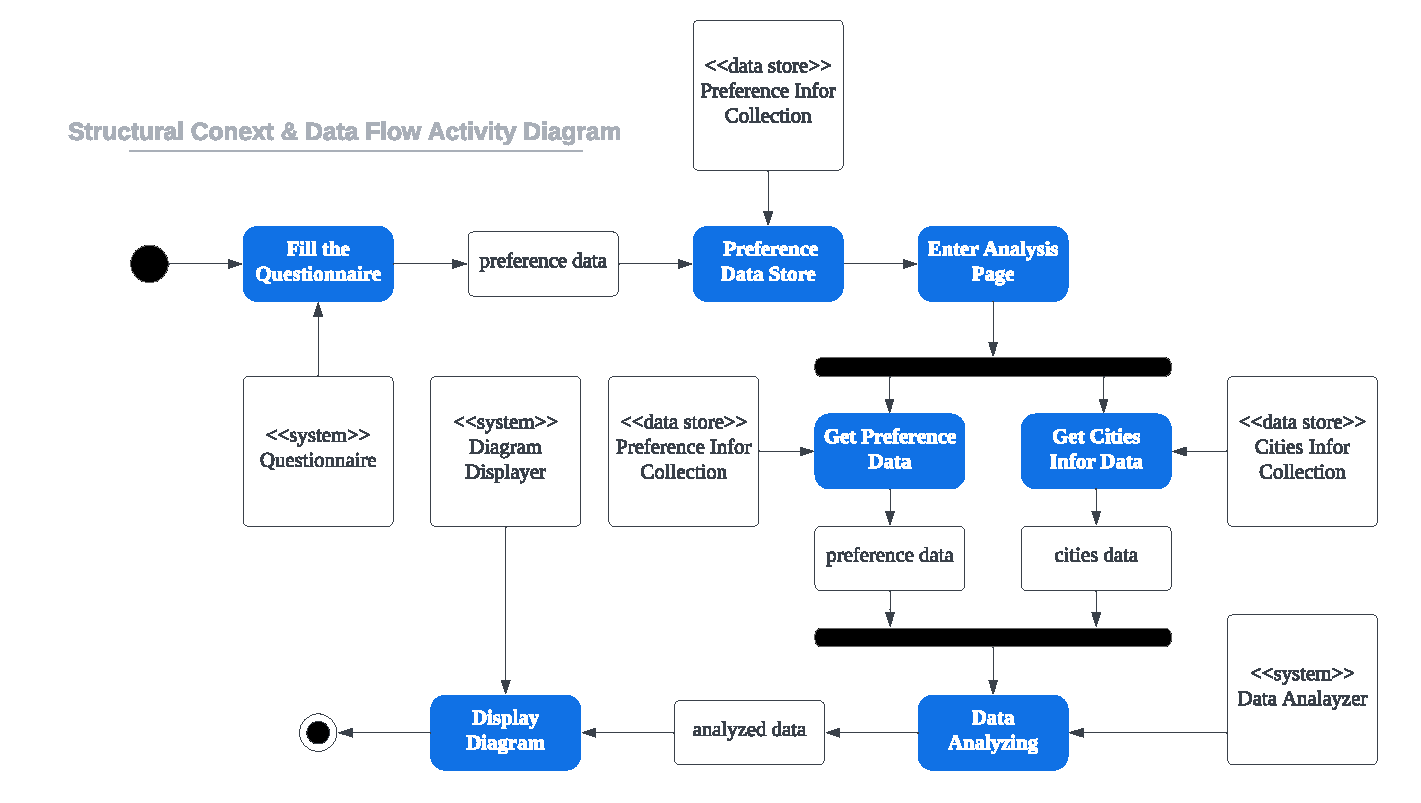
\includegraphics[width=1.0\textwidth]{diagram_data_flow.pdf}}
\caption{The structural context and data flow of analysis diagram task.}
\label{diagram_data_flow}
\end{figure*}

\subsubsection{\textbf{Structural Conext and Task Data Flow}}

\textbf{}

In this section, we discuss the data flow processing by Figure \ref{diagram_data_flow}. Meanwhile, we show the roles these objects play in the data flow processing, which describes the structural context of the Analysis Diagram task.

The user fills out the questionnaire on the questionnaire web page with the help of the questionnaire system. The Preference Information Collection saves the user's preference information for further analysis. Subsequently, the user enters the analysis page, which calls the Get Data Functions of Preference Information Collection and Cities Information Collection simultaneously. The preference data and city data are sent to the Data Analyzer for data analysis. Finally, the Diagram Displayer shows the data diagram based on analyzed data.


\begin{figure*}[htbp]
\centerline{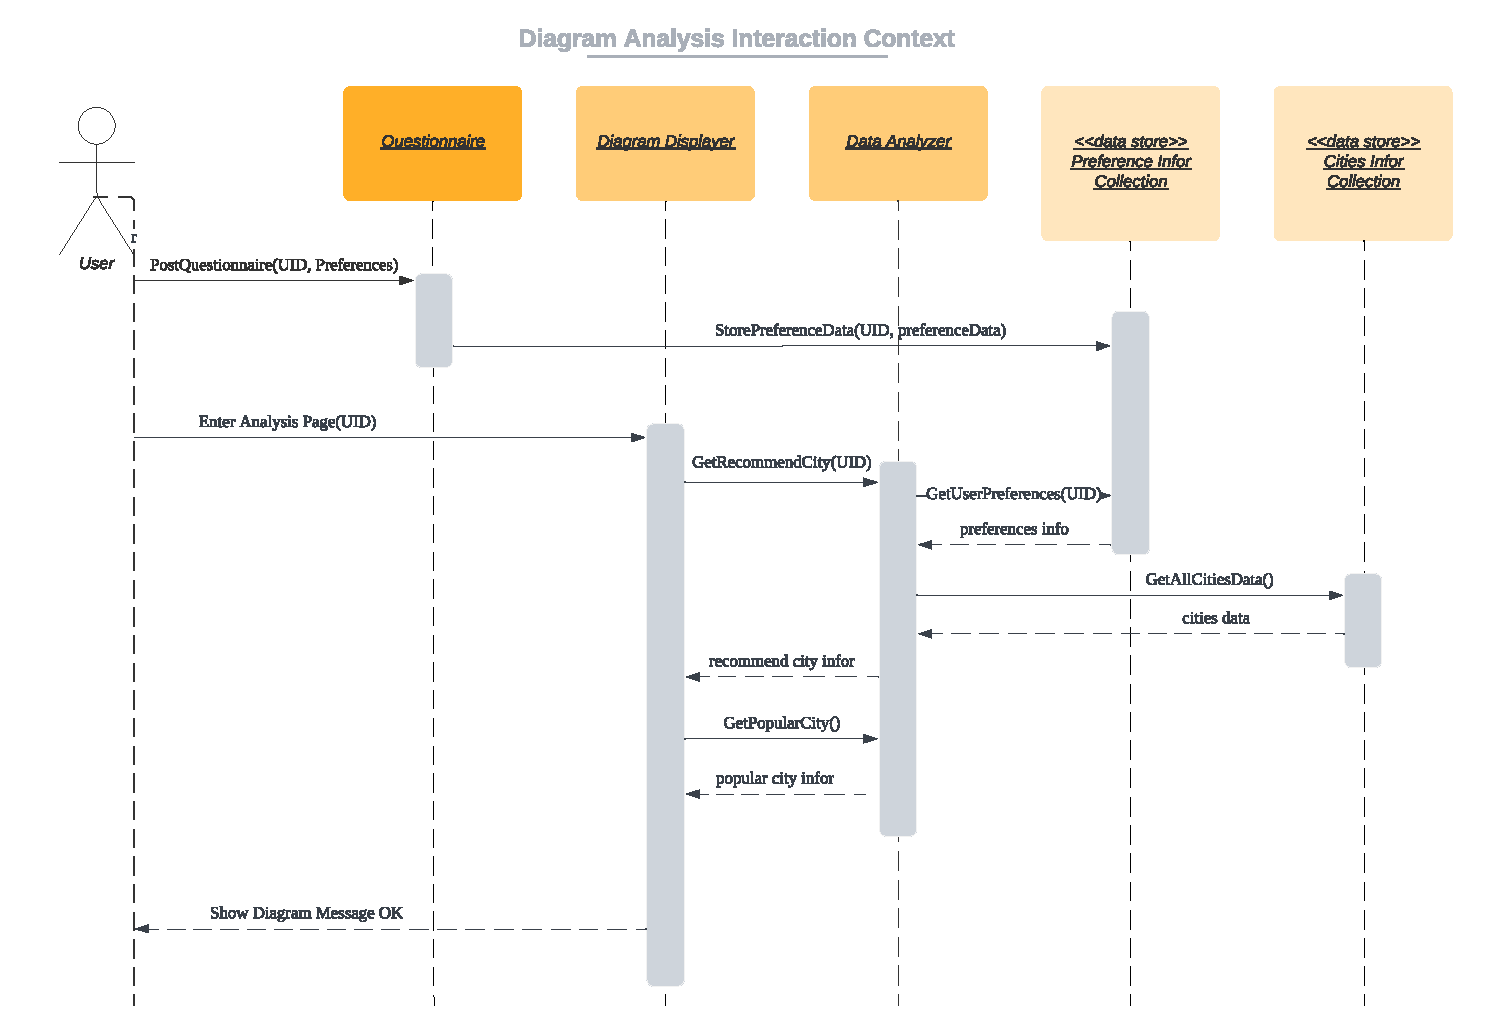
\includegraphics[width=1.0\textwidth]{diagram_interaction_context.pdf}}
\caption{The interaction context of analysis diagram task.}
\label{diagram_interaction}
\end{figure*}

\subsubsection{\textbf{Interaction Conext }}

\textbf{}

The sequence diagram in Figure \ref{diagram_interaction} shows the interaction context of this task. 

The user fills out the questionnaire and calls the PostQuestionnaire function of the Questionnaire object. The Questionnaire object calls the StorePreferenceData function provided by the Preference Infor Collection object to save the preference data into the database. 

Then the user clicks the 'recommend' button on the home page and calls the EnterAnalysisPage function, which is provided by the Diagram Displayer object. The Diagram Displayer object makes a request to the Data Analyzer for the recommendation information. The Data Analyzer gets the user preference data from the Preference Infor Collection object according to the UID. Meanwhile, all city data is gained from the Cities Infor Collection object. The Data Analyzer processes a recommendation algorithm based on these data and feeds back the recommended city information and popular city information. The Diagram Displayer shows the data diagram and returns an OK message to the user.


\begin{figure}[htbp]
\centerline{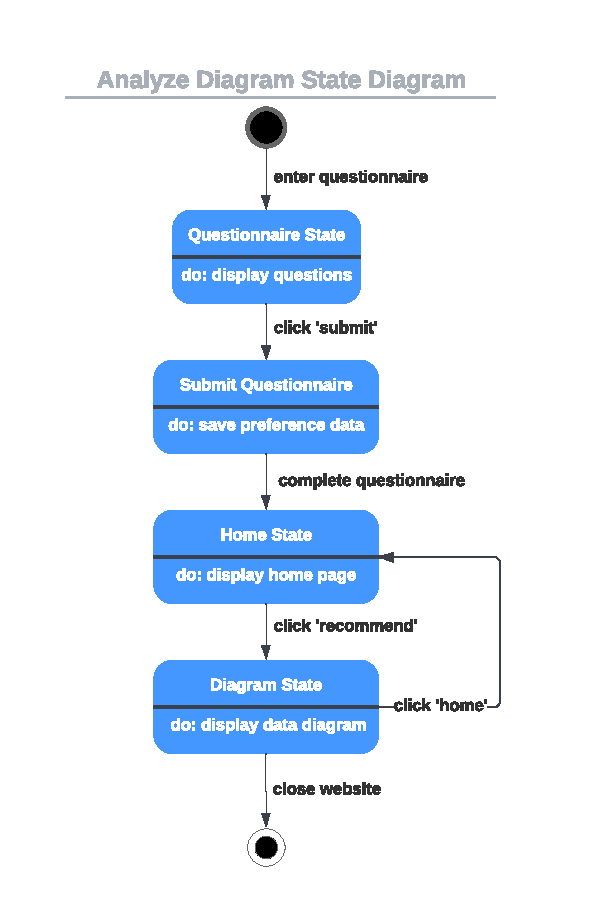
\includegraphics[width=0.5\textwidth]{diagram_state_diagram.pdf}}
\caption{The state diagram of analysis diagram task.}
\label{diagram_state_diagram}
\end{figure}


\subsubsection{\textbf{Behavior Conext }}

\textbf{}

The state diagram in figure \ref{diagram_state_diagram} shows the behavior context of this task. The state transition is simple and most functions in this task process data invisible to users. We divide the state according to the function of the web page. In this section, we only care about the states related to the analysis diagram task.

The user enters the questionnaire web page, the system enters into the Questionnaire State. The Questionnaire State displays the multiple psychological questions for users. After finishing the questionnaire, the system saves the preference data into the database. Subsequently, the website comes back to the home page and the system enters the home state. When the user clicks the 'recommend' button, the website jumps to the Analysis Diagram Page. After the system completes the recommendation, the Analysis Diagram Page displays the data diagram. 



\section{\textbf{Uncompleted Task Design }}


\subsubsection{\textbf{Task Conext }}


\subsubsection{\textbf{Structural Conext }}


\subsubsection{\textbf{Interaction Conext }}


\subsubsection{\textbf{Behavior Conext }}



\section{\textbf{Progress Evaluation \& Analysis }}









\end{document}
